\documentclass[border=4pt]{standalone}
\usepackage{amsmath}
\usepackage{tikz}
\usetikzlibrary{arrows.meta}

\definecolor{figblue}{RGB}{91,155,213}
\definecolor{figorange}{RGB}{237,125,49}
\definecolor{figgold}{RGB}{255,192,0}
\definecolor{figgreen}{RGB}{112,173,71}

\newcommand{\tftbdry}{%
  \draw[thick](0,0)rectangle(4,4);
  \draw[gray!25,very thin](2,0)--(2,4)(0,2)--(4,2);
  \fill[black!55](-0.10,1.90)--(0.10,1.90)--(0,2.10)--cycle;
  \fill[black!55](3.90,1.90)--(4.10,1.90)--(4,2.10)--cycle;
  \fill[black!55](1.90,-0.10)--(1.90,0.10)--(2.10,0)--cycle;
  \fill[black!55](1.90,3.90)--(1.90,4.10)--(2.10,4)--cycle;
  \foreach \v/\lab in {0/{0},2/{\pi},4/{2\pi}}{%
    \draw(\v,0)--(\v,-0.12);
    \draw(0,\v)--(-0.12,\v);\node[left,font=\tiny]at(-0.12,\v){$\lab$};
  }
  \foreach \v/\lab in {0/{0},4/{2\pi}}{%
    \node[below,font=\tiny]at(\v,-0.15){$\lab$};
  }
  \node[font=\scriptsize]at(2,-0.62){$\theta_1$};
  \node[left,font=\scriptsize]at(-0.55,2){$\theta_2$};
}
\newcommand{\tftAB}{%
  \fill[figblue!50]  (0.5,0.5)circle(0.318);
  \fill[figorange!55](2.5,2.5)circle(0.318);
  \node[font=\tiny]at(0.5,0.48){$A_0$};
  \node[font=\tiny]at(2.5,2.48){$A_1$};
}

\begin{document}
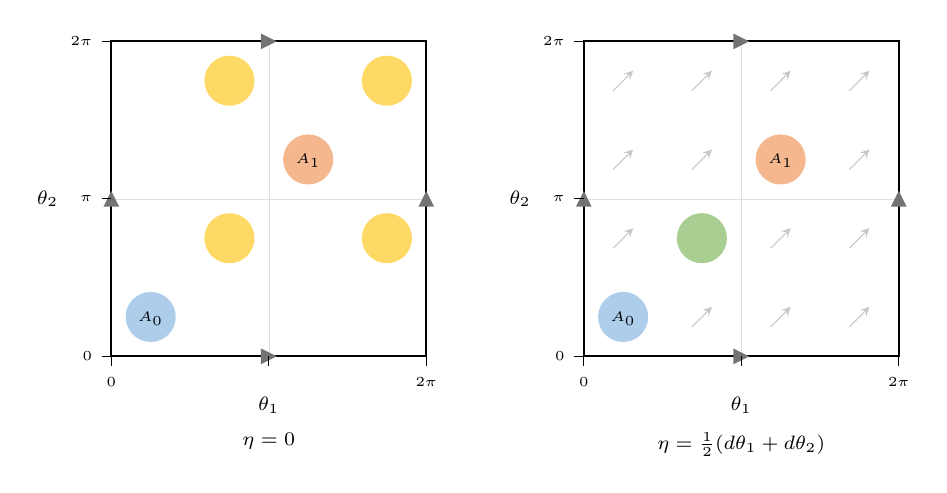
\begin{tikzpicture}[scale=1.0]
  \begin{scope}
    \tftbdry
    \fill[figgold!60](1.5,1.5)circle(0.318);
    \fill[figgold!60](3.5,3.5)circle(0.318);
    \fill[figgold!60](1.5,3.5)circle(0.318);
    \fill[figgold!60](3.5,1.5)circle(0.318);
    \tftAB
    \node[below,font=\scriptsize]at(2,-0.85){$\eta=0$};
  \end{scope}
  \begin{scope}[xshift=6cm]
    \tftbdry
    \foreach \xi in {0.5,1.5,2.5,3.5}{%
      \foreach \yi in {0.5,1.5,2.5,3.5}{%
        \draw[->,>=stealth,black!22,thin](\xi-0.127,\yi-0.127)--(\xi+0.127,\yi+0.127);
      }
    }
    \fill[figgreen!60](1.5,1.5)circle(0.318);
    \tftAB
    \node[below,font=\scriptsize]at(2,-0.85){$\eta=\tfrac12(d\theta_1+d\theta_2)$};
  \end{scope}
\end{tikzpicture}
\end{document}
